
%\RequirePackage{pdf15}

\documentclass{beamer}

\usepackage[utf8]{inputenc}

\usepackage{mystyle}

\usepackage{tikz}
\usepackage{pgfplots}
\usepackage{subcaption}

\usepackage{natbib}
\bibliographystyle{apalike}
%\usepackage[style=authortitle,backend=biber]{biblatex}
%\addbibresource{anthology.bib}
%\addbibresource{emnlp2020.bib}
\renewcommand{\footnotesize}{\scriptsize}

\newcommand{\bigCI}{\mathrel{\text{\scalebox{1.07}{$\perp\mkern-10mu\perp$}}}}

\usepackage{tikz-dependency}
\usetikzlibrary{shapes.arrows, positioning, fit, bayesnet,
    arrows,backgrounds,patterns,matrix,calc,shadows,plotmarks,
    shapes,positioning,automata,positioning,spy,scopes,chains,decorations,decorations.pathreplacing}

\newcommand{\FancyUpArrow}{
\begin{tikzpicture}[baseline=-0.3em]
\node[single arrow,draw,rotate=90,single arrow head extend=0.2em,inner
ysep=0.2em,transform shape,line width=0.05em,top color=green,bottom color=green!50!black] (X){};
\end{tikzpicture}}
\newcommand{\FancyDownArrow}{
\begin{tikzpicture}[baseline=-0.3em]
\node[single arrow,draw,rotate=-90,single arrow head extend=0.2em,inner
ysep=0.2em,transform shape,line width=0.05em,top color=red,bottom color=red!50!black] (X){};
\end{tikzpicture}}

\AtBeginSection[]{
  \begin{frame}
  \vfill
  \centering
  \begin{beamercolorbox}[sep=8pt,center,shadow=true,rounded=true]{title}
    \usebeamerfont{title}\insertsectionhead\par%
  \end{beamercolorbox}
  \vfill
  \end{frame}
}

% quotes
\usepackage[style=british]{csquotes}

\def\signed #1{{\leavevmode\unskip\nobreak\hfil\penalty50\hskip1em
  \hbox{}\nobreak\hfill #1%
  \parfillskip=0pt \finalhyphendemerits=0 \endgraf}}

\newsavebox\mybox
\newenvironment{aquote}[1]
  {\savebox\mybox{#1}\begin{quote}\openautoquote\hspace*{-.7ex}}
  {\unskip\closeautoquote\vspace*{1mm}\signed{\usebox\mybox}\end{quote}}

%Information to be included in the title page:
\title{Word Games}
\author{J Chiu}

\setbeamertemplate{navigation symbols}{} 
\setbeamertemplate{footline}[frame number]

\begin{document}

\begin{frame}[plain]
\titlepage
\end{frame}

\begin{frame}
\frametitle{Dialogue and information gathering}
\begin{itemize}
\item Resolve ambiguity and coordinate through dialogue
\item OneCommon: Interactive, symmetric reference game
    \begin{itemize}
    \item Isolates info gathering (and coordination)
    \item Environment (dots) are completely static
    \item Dynamism comes from dialogue only
    \end{itemize}
\item 20 questions with symmetric information constraints
\end{itemize}
\end{frame}

\begin{frame}
\frametitle{Previous SotA}
\begin{itemize}
\item Purely supervised
    \begin{itemize}
    \item Upper-bounded by performance of demonstrators
    \end{itemize}
\item Uncalibrated beliefs: overconfidence
    \begin{itemize}
    \item Pushes for to select a dot that will not work
    \end{itemize}
\item Research goal: Improve supervised models via model-based planning
\end{itemize}
\end{frame}


\begin{frame}
\frametitle{Fixing strategy with planning}
\begin{itemize}
\item Prior: Fully supervised neural encoder-decoder
    \begin{itemize}
    \item Encode past interactions with a neural net
    \item Generate what to say with a neural net
    \item Brittle strategy, less brittle language
    \end{itemize}
\item Next: Model-based planning
    \begin{itemize}
    \item Choose what to say by imagining how partner would respond
    \item Say utterance with best expected outcome
    \item Potentially stronger player than expert demonstrations
    \end{itemize}
\end{itemize}
\end{frame}

\begin{frame}
\frametitle{Challenges in model-based planning}
\begin{itemize}
\item Partner modeling is hard
    \begin{itemize}
    \item Variable amount of information in utterances
    \item High entropy demonstration strategies
    \end{itemize}
\item Multi-turn planning
    \begin{itemize}
    \item Accuracy of planning depends greatly on the partner model
    \item Errors from the partner model will compound over time\footnote{
        Errors in planning will be a result of compounding partner model errors
            on top of search error.
    }
    \end{itemize}
\item Single-turn planning
    \begin{itemize}
    \item Removes compounding errors
    \item Must optimize a dialogue progress heuristic: uncertainty reduction
    \item Requires belief with uncertainty
    \item Still requires accurate partner model\footnote{
        Belief is function of dialogue history and partner model.
    }
    \end{itemize}
\item Research question: Can we improve partner modeling for planning
    by simplifying partner responses?
\end{itemize}
\end{frame}

\begin{frame}
\frametitle{Planning}
\begin{itemize}
\item Partner response depends on utterance and conversation history
    \begin{itemize}
    \item First history $h_0 = \text{dots you can see}$
    \item History $h_t$, utterance $u$, response $r$
    \item Next history $h_{t+1} = (h_t, u, r)$
    \end{itemize}
\begin{center}
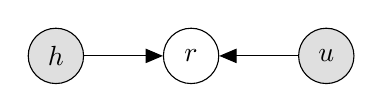
\begin{tikzpicture}
\node[obs] (h) {$h$};
\node[latent, right=of h] (r) {$r$};
\node[obs, right=of r] (u) {$u$};

\path (h) edge[->] (r);
\path (u) edge[->] (r);
\end{tikzpicture}
\end{center}
\item Plan by imagining partner response $r$
$$\min_{u} \Es{p(r \mid h, u)}{\text{Cost}(h, u, r)}$$
    \begin{itemize}
    \item Produce utterances from prior model and rerank
    \end{itemize}
\item Cost should approximate dialogue progress
    \begin{itemize}
    \item Goal of dialogue is information gathering and coordination
    \item Focus on information gathering
    \end{itemize}
\item Cost should be a function of belief
\end{itemize}
\end{frame}

\begin{frame}
\frametitle{Planning with Belief}
\begin{itemize}
\item Introduce belief $p(s \mid h)$
    \begin{itemize}
    \item State $s$ is what dots partner can also see
    \item Response model $p(r \mid h,u,s)$ now has more conditioning
    \end{itemize}
\begin{center}
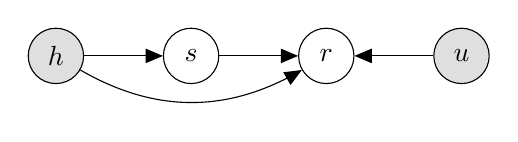
\begin{tikzpicture}
\node[obs] (h) {$h$};
\node[latent, right=of h] (s) {$s$};
\node[latent, right=of s] (r) {$r$};
\node[obs, right=of r] (u) {$u$};

\path (h) edge[->, bend right=30] (r);
\path (h) edge[->] (s);
\path (s) edge[->] (r);
\path (u) edge[->] (r);
\end{tikzpicture}
\end{center}
\item Incorporate belief in planning
$$\min_{u} \Es{p(r \mid h, u, s)p(s \mid h)}{\text{Uncertainty}(p(s \mid h, u, r))}$$
\item Obtain belief posterior via belief update
$$p(s \mid h, u, r) = \frac{p(r \mid h, u, s)p(s \mid h)}{\sum_s p(r\mid h,u,s)p(s \mid h)}$$
\end{itemize}
\end{frame}

\begin{frame}
\frametitle{Partner response model}
\begin{itemize}
\item Static latent state $s$: which dots do they also see
    \begin{itemize}
    \item Alternative: actual field of view
    \item Pick $s$ that is observed during training so we can keep
        all models supervised
    \end{itemize}
\item Uniform prior $p(s)$ over 7 choose 4 dots partner also sees
\item Partner response model $p(r_t \mid u_{1:t},r_{1:t-1}, s)$
    \begin{itemize}
    \item History $h_t = (u_{1:t-1}, r_{1:t-1})$
    \end{itemize}
\begin{center}
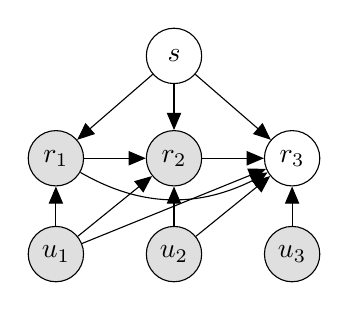
\begin{tikzpicture}
\node[latent] (s) {$s$};
\node[obs] at (-1.5,-1.3) (o1) {$r_1$};
\node[obs] at (0, -1.3) (o2) {$r_2$};
\node[latent] at (1.5,-1.3) (o3) {$r_3$};

\node[obs, below=.5cm of o1] (a1) {$u_1$};
\node[obs, below=.5cm of o2] (a2) {$u_2$};
\node[obs, below=.5 of o3] (a3) {$u_3$};

\edge {s} {o1};
\edge {s} {o2};
\edge {s} {o3};

\edge {a1} {o1};
\edge {a1} {o2};
\edge {a1} {o3};
\edge {a2} {o2};
\edge {a2} {o3};
\edge {a3} {o3};

\edge {o1} {o2};
\path (o1) edge[->, bend right=30] (o3);
\edge {o2} {o3};
\end{tikzpicture}
\end{center}
\end{itemize}
\end{frame}

\begin{frame}
\frametitle{Response model: Informativity}
\begin{itemize}
\item Example exchange
    \begin{itemize}
    \item Action: Do you see a red dot?
    \item Observation: No, but I see a blue one.
    \end{itemize}
\item Utterances are multifaceted
    \begin{itemize}
    \item Responses contain more information than asked
    \item New information injected by partner, not constrained
    \item Difficult to model new information
    \end{itemize}
\item Introduce informativity as another variable
\item Make worst-case assumption about informativity \textbf{during planning}
    \begin{itemize}
    \item Assume a limit on number of bits transmitted
    \item Conservative lower bound on uncertainty reduction / dialogue progress
    \end{itemize}
\end{itemize}
\end{frame}

\begin{frame}
\frametitle{Incorporating informativity}
\begin{itemize}
\item Add partner-level informativity $i$ to response model
$p(r \mid h, u, s, i)$
    \begin{itemize}
    \item Determines partner willingness to give more information
    \item More information improves game-play
    \end{itemize}
\item Introduce uncertainty set over $i \in [\text{low}, \text{high}]$
$$\min_{u}\min_{i\in[\text{low},\text{high}]}
    \Es{p(r \mid h, u, s, i)p(s \mid h)}{\text{Uncertainty}(p(s \mid h, u, r))}$$
\item Optimize worst-case informativity $i = \text{low}$
\item Constrain informativity in response via discrete coding
\end{itemize}
\end{frame}

\begin{frame}
\frametitle{Limiting informativity with discrete coding}
\begin{itemize}
\item Compress response into discrete code $z \in [K]$
\item Use variational information bottleneck (VIB)\footnote{\citet{vib}}
\item Optimize mutual information objective\footnote{Closely related to the approach of \citet{li}}
    \begin{itemize}
    \item Focus code $z$ on response to new information introduced by utterance $u$
    \item But limit the information shared with response $r$ and history $h$
    \end{itemize}
$$\max_\theta I(z, u; \theta) - \beta I(z, r; \theta) - \gamma I(z, h; \theta)$$
\item Lagrange multipliers $\beta,\gamma$
\item Plan with response model $p(z \mid h, u, s)$ instead of $r$
\end{itemize}
\end{frame}

\begin{frame}
\frametitle{Belief update}
\begin{itemize}
\item Performing the belief update with $z$ instead of $r$ would lose information
\item Use original model $p(r \mid h, u, s)$ to update belief?
    \begin{itemize}
    \item May run into original possible issue of poor calibration
    \end{itemize}
\item Learn another discrete representation of $r$ that does not aim
    to disentangle
    \begin{itemize}
    \item Need as baseline for model with $z$
    \item Likely adequate when combined with mentions
    \end{itemize}
\end{itemize}
\end{frame}

\begin{frame}
\frametitle{Summary}
\begin{itemize}
\item Goal: Show (partner) model-based planning works for dialogue with
    purely supervised components
    \begin{itemize}
    \item Single-turn planning for limiting compounding model errors
    \item Belief-based heuristic for measuring dialogue progress
    \item Response coding for conservative planning
    \end{itemize}
\end{itemize}
\end{frame}

\begin{frame}
\frametitle{Belief unit tests}
Belief calibration: check belief dynamics on static conversations.
\begin{itemize}
\item Diminishing returns
    \begin{itemize}
    \item Ask the same question twice (rephrased) should not change belief
    \item Asking about the same dot should have diminishing
        uncertainty reduction
    \end{itemize}
\item Updates are conservative
    \begin{itemize}
    \item Require multiple positive answers
        to diff questions before being certain about a dot
    \end{itemize}
\item High probability after confirming all neighbouring dots
\end{itemize}
\end{frame}

\begin{comment}
\item Follow-up questions improve belief
    \begin{itemize}
    \item Want one case where first (uncertain) answer results in less information
        and vice versa
    \end{itemize}
\item Multiple partner dots satisfy question
    \begin{itemize}
    \item Still a positive response, might be same as single satisfy
    \item Next preferred utterance should be a follow-up in both multiple and
        single satisfy
    \end{itemize}
\end{comment}

\begin{frame}
\frametitle{Extrinsic evaluation: Selfplay}
Compare to prior work (without belief)
\begin{itemize}
\item Success rate
    \begin{itemize}
    \item Should be higher
    \end{itemize}
\item Efficiency (success / num turns)
    \begin{itemize}
    \item Possibly higher because more success, but more turns
    \end{itemize}
\item Number of repeated mentions
    \begin{itemize}
    \item Should be higher if policy more conservative
    \end{itemize}
\end{itemize}
\end{frame}

\begin{frame}
\frametitle{Questions}
\begin{enumerate}
\item How do we measure belief calibration?
    \begin{itemize}
    \item Unit tests examining conservativity of beliefs
    \end{itemize}
\item How calibrated are the belief updates using various response representations?
    \begin{itemize}
    \item Too much information (ie full word response) results in low probability
        to responses, which results in a large belief update = optimism
    \item Not enough information = conservative
    \end{itemize}
\item How well can we produce a range of utterances to search over?
\end{enumerate}
\end{frame}

\begin{frame}
\frametitle{Hypothesis}
\begin{itemize}
\item High information response representation
    \begin{itemize}
    \item Calibrated policy (assuming accurate model)
    \item Hard to model responses
    \end{itemize}
\item Low information response representation
    \begin{itemize}
    \item Conservative policy (assuming accurate model)
    \item Easy to model responses
    \end{itemize}
\item Prefer conservative + accuracy response model over
    inaccurate response model
\end{itemize}
\end{frame}

\begin{frame}
\frametitle{Response representations}
\begin{itemize}
\item Words in response
    \begin{itemize}
    \item Full response
    \item First $k$ words of response
    \end{itemize}
\item Dot mentions
    \begin{itemize}
    \item All dot groups mentioned in response
    \item First $k$ dot groups mentioned in response
    \end{itemize}
\item Discrete encoding
    \begin{itemize}
    \item K-means cluster of sentence rep
    \item Specialized cluster (information bottleneck)
    \end{itemize}
\item Continuous encoding
    \begin{itemize}
    \item Sentence rep
    \item Specialized encoding (information bottleneck)
    \end{itemize}
\end{itemize}
\end{frame}

\begin{frame}
\frametitle{Experiments}
\begin{itemize}
\item Evaluate response representations on unit tests and selfplay
\item Binary matrix of representation x unit test property
\item Main unit tests
    \begin{itemize}
    \item Diminishing returns
    \item Conservativity
    \item High probability
    \end{itemize}
\item Representations
    \begin{itemize}
    \item Words
    \item Dots
    \item Learned (discrete, continuous)
    \end{itemize}
\item Consider highest and lowest information representations,
    work our way in
    \begin{itemize}
    \item Hypothesize that best point is in between first dot and all dots
    \end{itemize}
\end{itemize}
\end{frame}

\begin{frame}
\frametitle{Experiment 1}
Evaluate word response models on belief unit tests
\begin{itemize}
\item Belief representations
    \begin{itemize}
    \item Full response
    \item First $k$ words
    \end{itemize}
\item Hypothesis
    \begin{itemize}
    \item Full response will fail all unit tests
    \item First $k$ will fail high probability test.
        Too conservative due to missing information
    \end{itemize}
\item Outcomes
    \begin{itemize}
    \item Full is too optimistic, motivating different representations
        for exploring more conservative belief updates
    \item Full is conservative, which is a success. Method is general,
        just need to try it on other datasets
    \item First $k$ is too optimistic. This would indicate
        information hypothesis is wrong, and
        potential issues with any other subsequent representation approach.
    \end{itemize}
\end{itemize}
\end{frame}

\begin{frame}
\frametitle{Experiment 2}
Evaluate dot response models on belief unit tests
\begin{itemize}
\item Belief representations
    \begin{itemize}
    \item All dot mentions
    \item First $k$ dot mentions
    \end{itemize}
\item Hypothesis
    \begin{itemize}
    \item These might do okay on unit tests
    \item First $k=1$ often captures responses
    \end{itemize}
\item Outcomes
    \begin{itemize}
    \item First $k$ fails due to optimism,
        implies info hypothesis is wrong.
    \item First $k$ succeed, which gives an indication that
        a learned structured generalization has promise.
        If all also succeeds, same.
    \end{itemize}
\end{itemize}
\end{frame}

\begin{frame}
\frametitle{Experiment 3}
Evaluate learned discrete response models on belief unit tests
\begin{itemize}
\item We can tune the amount of information via number of clusters
\item If training goes well, should be able to get a
    fine-grained view of information - conservativity tradeoff
\item Belief representations
    \begin{itemize}
    \item K-means cluster on pretrained sentence rep
    \item Specialized cluster\footnote{\citet{li}}
    \end{itemize}
\item Hypothesis
    \begin{itemize}
    \item K-means might be pretty competitive, depending on sentence representations
    \item K-means should be conservative, since untuned sentence reps may not
        pick up relevant information
    \item Specialized clusters should do better than k-means with naive sentence rep
    \end{itemize}
\item Outcomes
    \begin{itemize}
    \item If any of these succeed, selfplay and try on another dataset
    \item If fail, end of line
    \end{itemize}
\end{itemize}
\end{frame}


\begin{frame}
\frametitle{End}
\end{frame}

\begin{frame}
\frametitle{Full planning details}
\begin{itemize}
\item Given history $h$,
we need to chose an action $a$ by optimizing heuristic utility
\begin{equation*}
\min_a C(h, a)
\end{equation*}
\item Cost $c$ = -information gain + utterance + pragmatic cost
    \begin{itemize}
    \item IG: Reduce uncertainty
    \item Utterance cost: Can't send a full paragraph
    \item Pragmatic cost: Want utterance to be accurate
    \end{itemize}
\item Ideally would estimate and optimize future reward directly
    \begin{itemize}
    \item Heuristic approximation of future reward $U$
    \item Limited-horizon planning to minimize impact of model error
    \end{itemize}
\end{itemize}
\end{frame}

\begin{frame}
\frametitle{Expected information gain}
\begin{itemize}
\item Maximizing expected information gain equivalent to minimizing uncertainty
$$\min_u \sum_r\sum_s
    \underbrace{p(r\mid h,u,s)}_{\text{response model}}
    \underbrace{p(s\mid h)}_{\text{belief}}
    \text{Uncertainty}(\underbrace{p(s \mid h,u,r)}_{\text{new belief}})$$
\end{itemize}
\end{frame}

\begin{frame}
\frametitle{Experiments}
\begin{itemize}
\item Mutual Friends
    \begin{itemize}
    \item Augment rule-based (prior work) to optimize info gain
    \item After OneCommon: Add neural on top
    \end{itemize}
\item OneCommon
    \begin{itemize}
    \item Use attributes = raw mention configurations
        \begin{itemize}
        \item Need belief / info gain / LR weights
        \item How to deal with redundancy? (i.e. correlation between features)
        \end{itemize}
    \item Learn latent refinement on top of mention configurations
    \end{itemize}
\end{itemize}
\end{frame}

\begin{frame}
\frametitle{Information gain issues}
\begin{itemize}
\item Best info gain could be to ask the same question twice
\item Usual fix: Limit to asking once only
\item Would be nice to have a principled way to deal with correlated
    features though
\end{itemize}
\centering
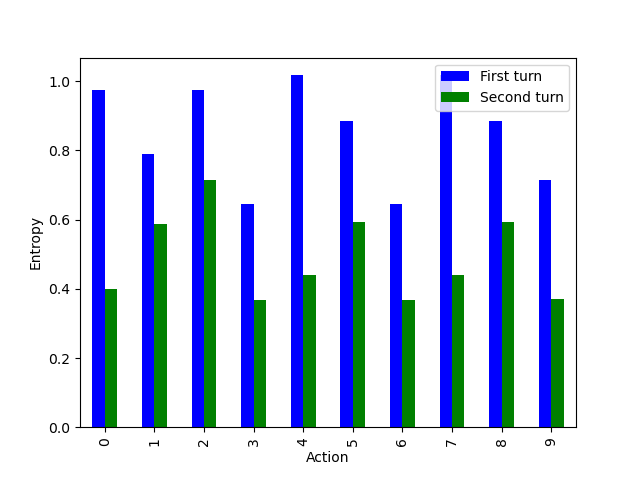
\includegraphics[height=2in]{src/entropy.png}
\begin{itemize}
\item Second turn after taking action with lowest entropy
\end{itemize}
\end{frame}

\begin{frame}
\frametitle{Related work: 20 questions}
\begin{itemize}
\item \citet{padmakumar}
    \begin{itemize}
    \item Attribute-based classification (string heuristic to map to description)
        + activate learning about attributes
    \item Info gain (on top of binary unweighted logistic regression) as feature for
        RL policy
    \end{itemize}
\item \citet{yu}
    \begin{itemize}
    \item Question-based classification (attributes)
    \item Learn weights of features
    \item Do not consider feature correlations
    \end{itemize}
\item More interesting language, symmetric setting
\item Learn weights, account for correlation
\item Symmetry, deal with unexpected features
\end{itemize}
\end{frame}

\begin{frame}
\frametitle{End}
\end{frame}


\begin{frame}
\frametitle{Concerns}
\begin{itemize}
\item Would a large LM solve all of this?
    \begin{itemize}
    \item Fine tune on small onecommon dataset, are there still repeats?
    \item Unlikely to solve strategy / over optimistism
    \end{itemize}
\end{itemize}
\end{frame}


\begin{frame}
\frametitle{Expected Information Gain}
\begin{align*}
IG(h, a) &= H(i \mid h) - \Es{p(o\mid h,a)}{H(i \mid h, a, o)}\\
\Es{p(o\mid h,a)}{H(i \mid h, a)} &= \sum_o\sum_{i'}p(o\mid h,a,i)p(i\mid h)H(i \mid h,a,o)
\end{align*}
\begin{itemize}
\item Equivalent to minimizing expected uncertainty after receiving a response
\item Cite Yu et al, White et al
\end{itemize}
\end{frame}

\begin{frame}[allowframebreaks]
\frametitle{Citations}
%\printbibliography
\bibliography{bib.bib}
\end{frame}

\begin{frame}
\frametitle{Games}

\begin{columns}
\begin{column}{0.5\textwidth}
\centering
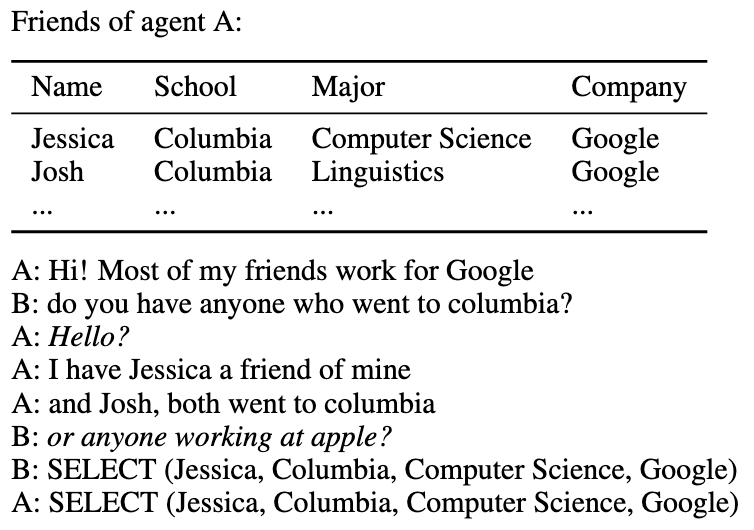
\includegraphics[width=2in]{img/mf.png}
\end{column}
\begin{column}{0.5\textwidth}
\centering
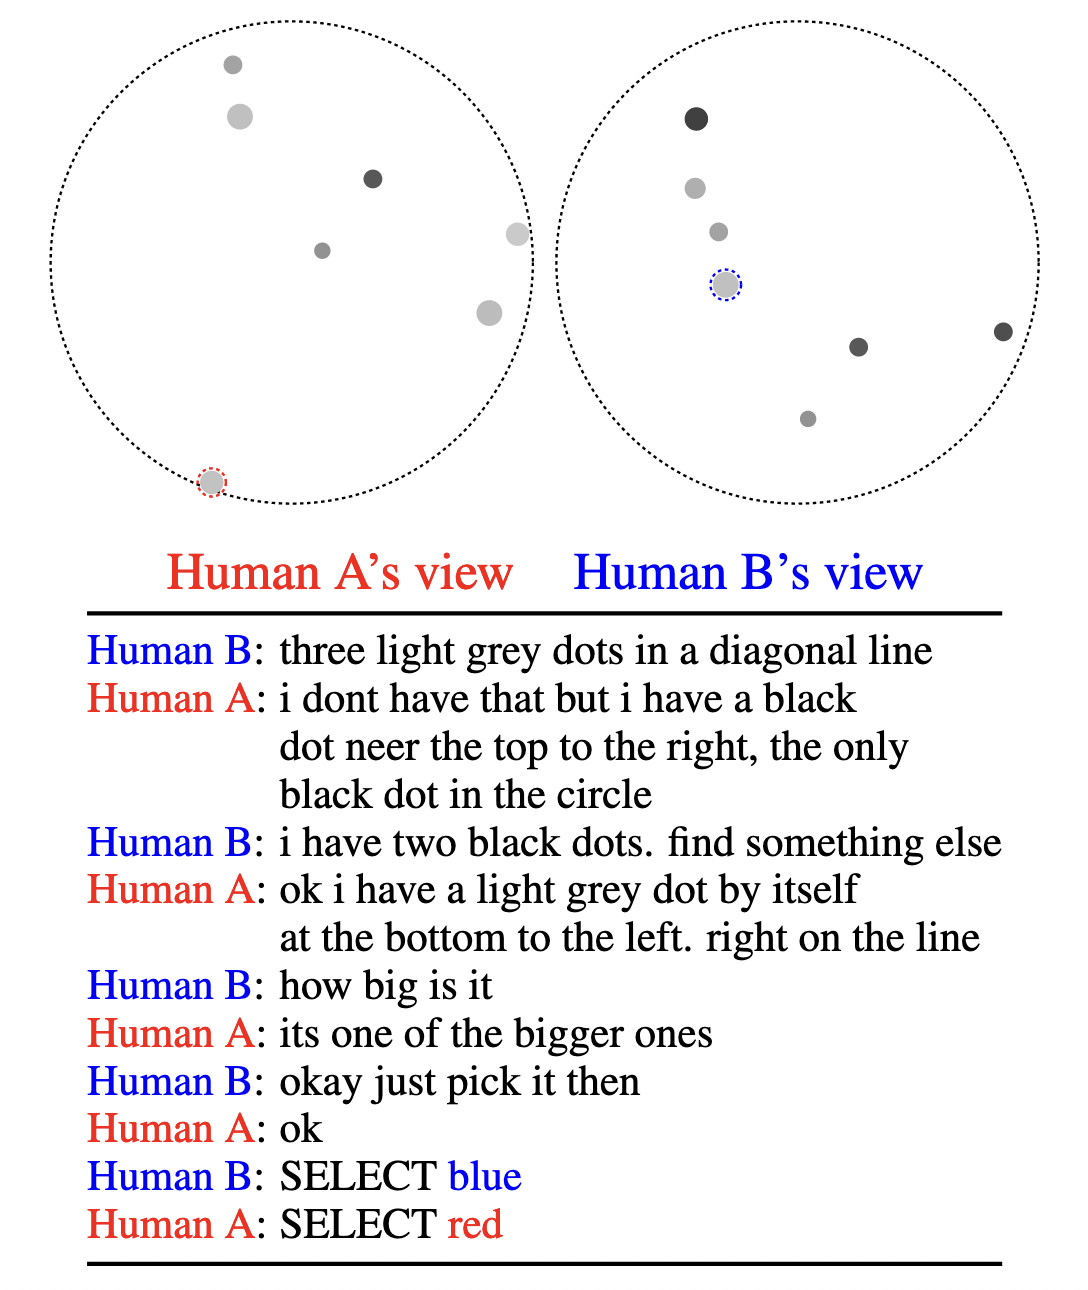
\includegraphics[width=2in]{img/oc.png}
\end{column}
\end{columns}

\vspace{2em}
\centering
Mutual Friends and OneCommon
\end{frame}

\begin{frame}
\frametitle{Issue: Poor neural reasoning}
From Mutual Friends: Neural + Human
\begin{itemize}
\item A: Know anyone who likes chess?
\item B: None of my friends like chess.
\item (conversation continues)
\item A: Crocheting?
\item B: None like crocheting.
\item A: Chess?
\item B: None like chess either, haha.
\end{itemize}
\end{frame}

\begin{frame}
\frametitle{Sample of prior work in model-based planning}
\begin{itemize}
\item 20 questions \citep{yu,padmakumar}
    \begin{itemize}
    \item Sym: Assymmetric questioner + answerer
    \item Turns: Multi-turn game
    \item Lang: Closed class answers (observations)
    \item Heur: Expected info gain heuristic
    \end{itemize}
\item EVPI \citep{rao,rao2}
    \begin{itemize}
    \item Sym: Assymmetric questioner + answerer
    \item Turns: No interaction, single turn game
    \item Lang: Open
    \item Heur: Expected utility heuristic
    \end{itemize}
\item RSA reference game \citep{khani}
    \begin{itemize}
    \item Sym: Symmetric
    \item Turns: Multi-turn game
    \item Lang: Symbolic language
    \item Heur: Bounded depth search
    \end{itemize}
\end{itemize}
\end{frame}

\begin{frame}
\frametitle{Conditioning in partner modeling}
\begin{itemize}
\item Assuming conditional independence $p(o \mid h, a, y) = p(o \mid a, y)$ is harmful
\item If you ask the same question twice, your belief changes both times!
    \begin{itemize}
    \item $p(\text{yes} \mid h = \emptyset, a=\text{red dot?},y)$ can vary depending on the latent $y$
    \item $p(\text{yes} \mid h = (\text{red dot?}, \text{yes}), a = \text{red dot?},y) = 1$,
        since we just asked!
    \end{itemize}
\item `Questions with correlated answers' and deficient observation model
    lead to uncalibrated beliefs, and therefore poor strategy
\item Contribution: relax independence assumption
    \begin{itemize}
    \item Let past obs vote on current one (weighted by action similarity)
    \item Probably solved by Transformers\footnote{Copy attention,
        depends on amount of data}
    \end{itemize}
\end{itemize}
\end{frame}

\begin{frame}
\frametitle{Example dialogue 1: Overconfidence}
\centering
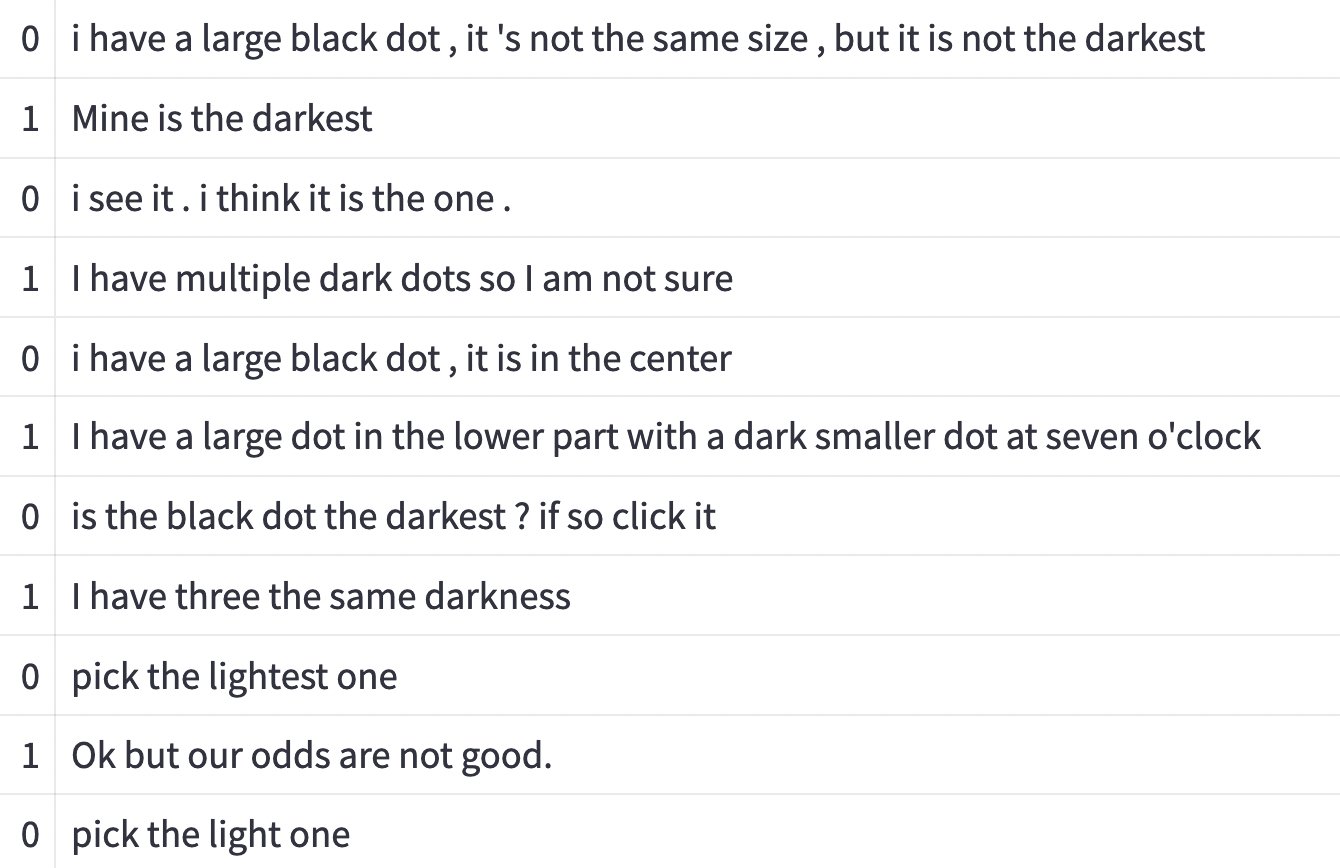
\includegraphics[width=\textwidth]{img/words1.png}
\end{frame}

\begin{frame}
\frametitle{Example dialogue 2: Overconfidence}
\centering
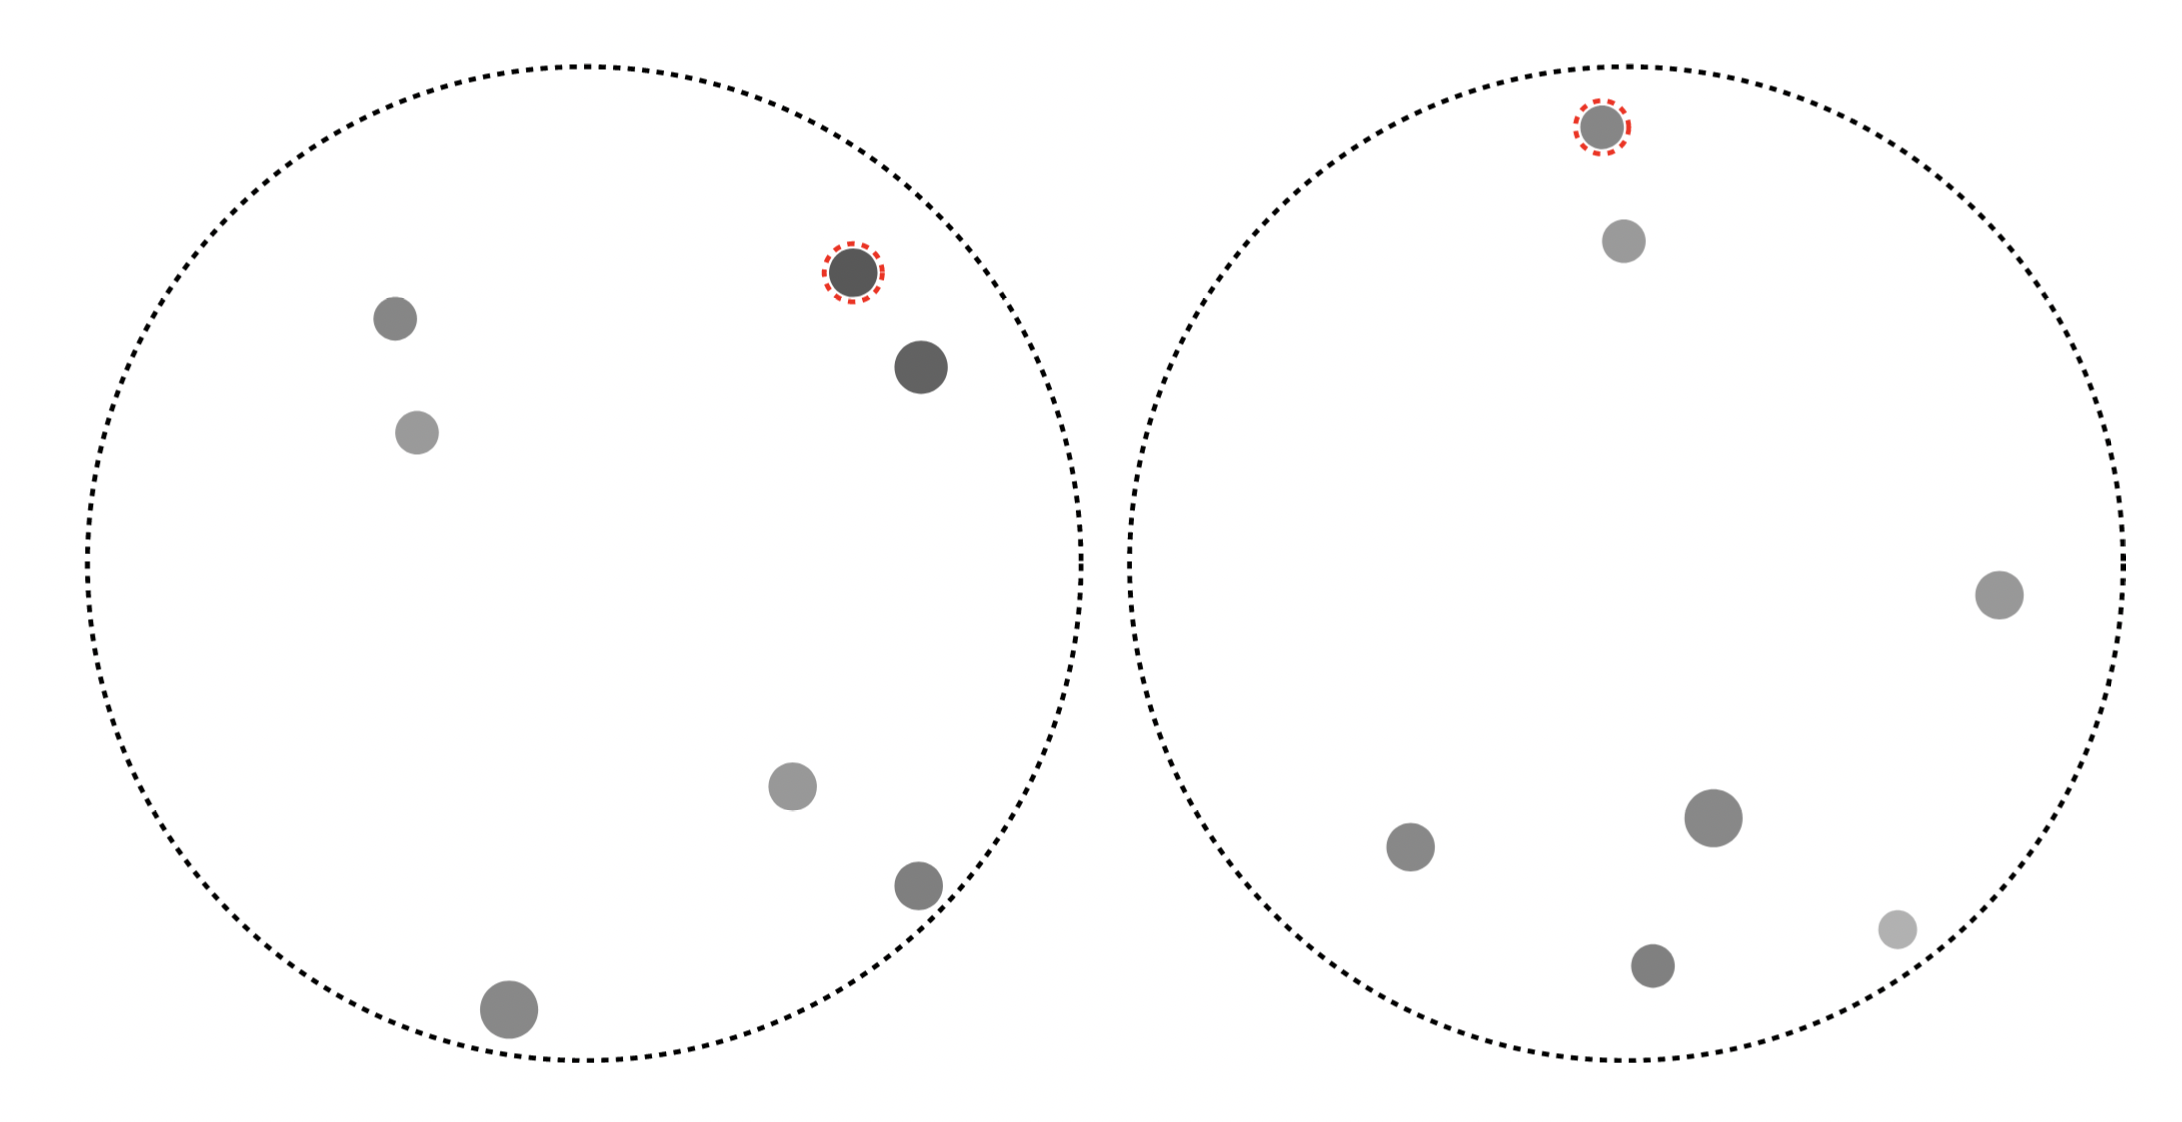
\includegraphics[width=0.75\textwidth]{img/dots2.png}
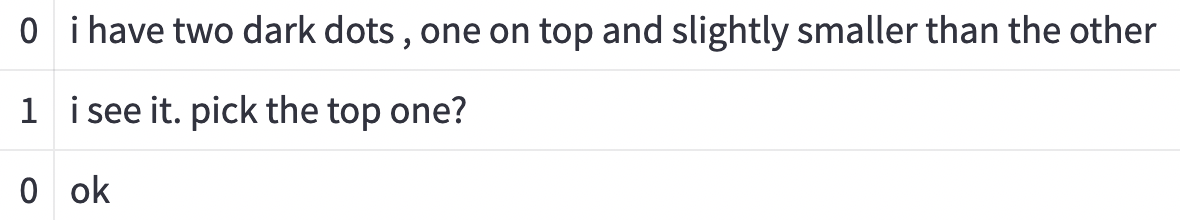
\includegraphics[width=\textwidth]{img/words2.png}
\end{frame}

\begin{frame}
\frametitle{Example dialogue 3: Good humans}
\centering
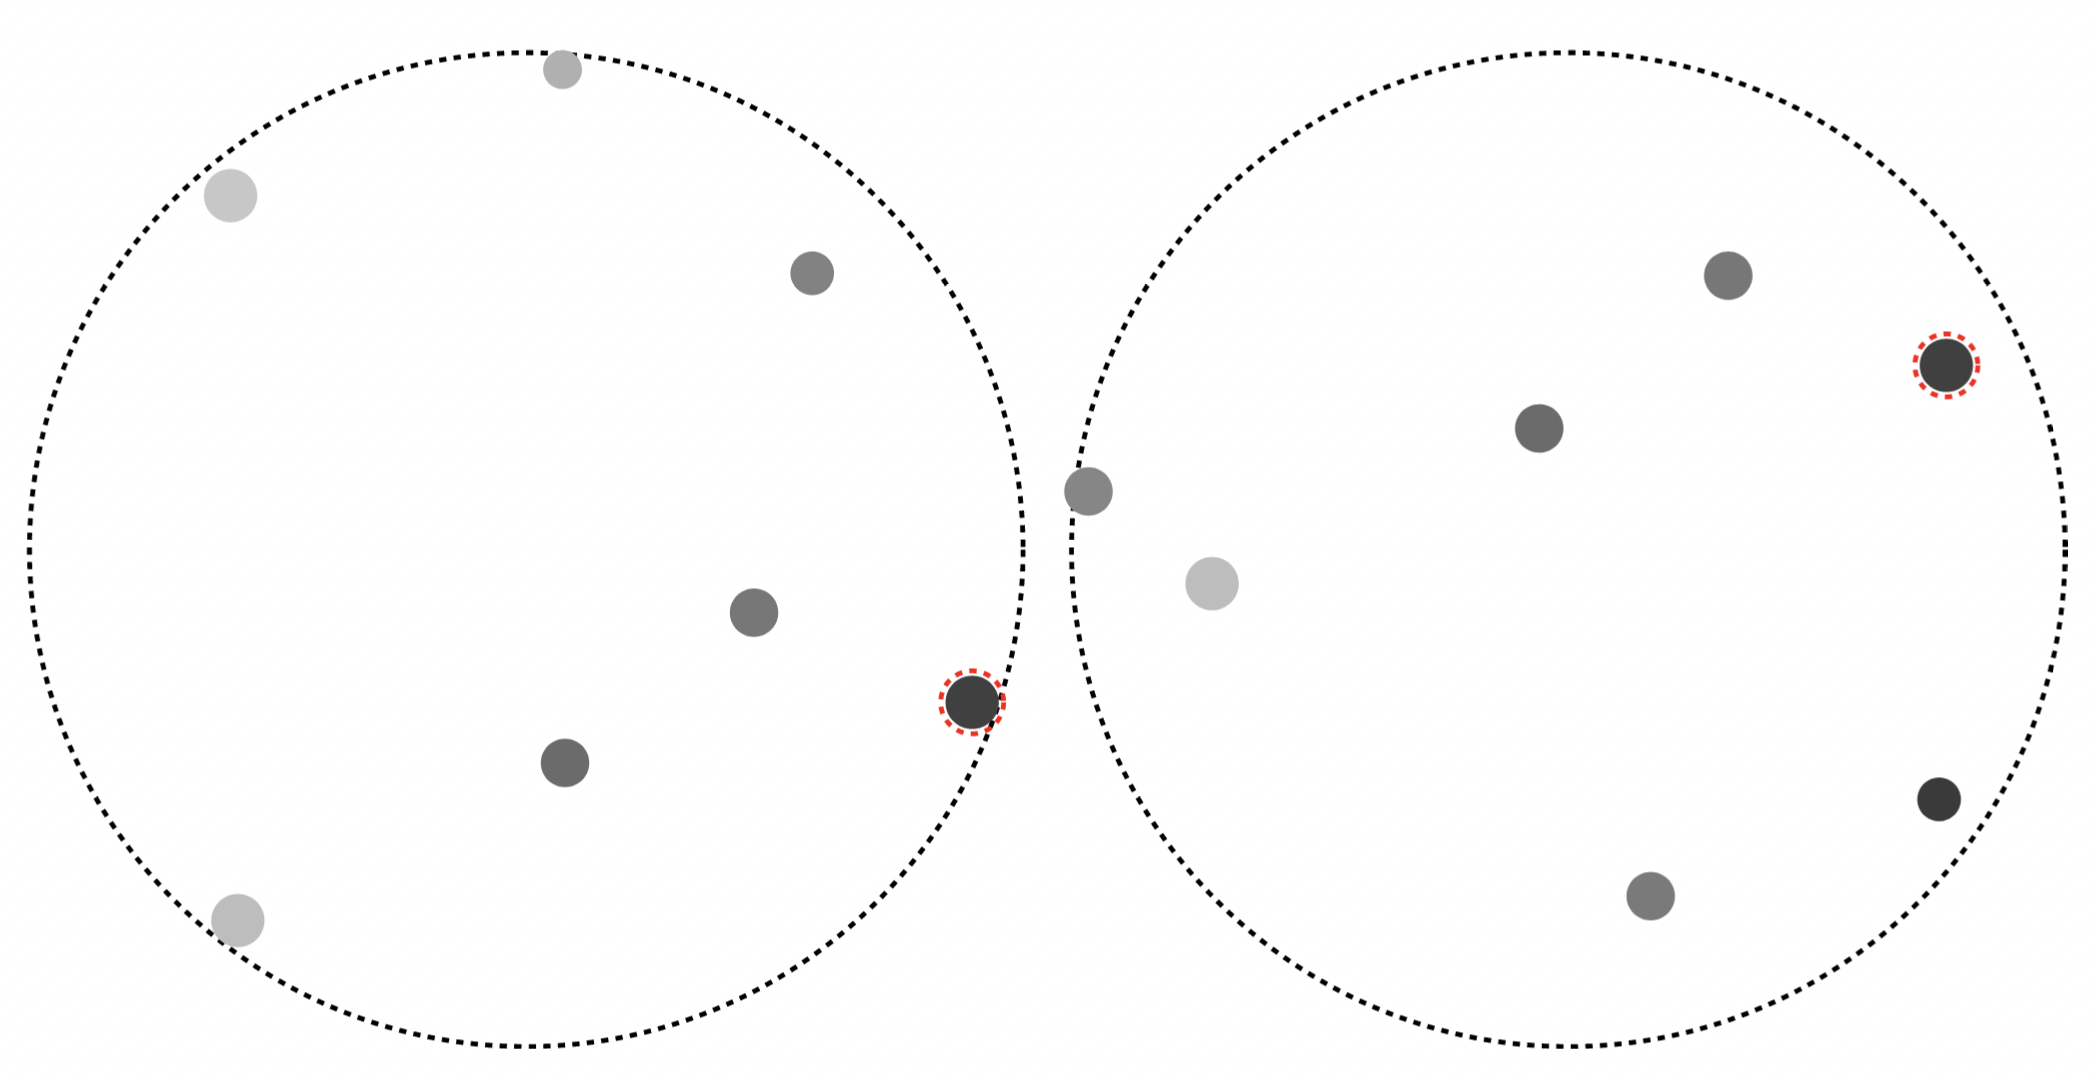
\includegraphics[width=0.75\textwidth]{img/dots3.png}
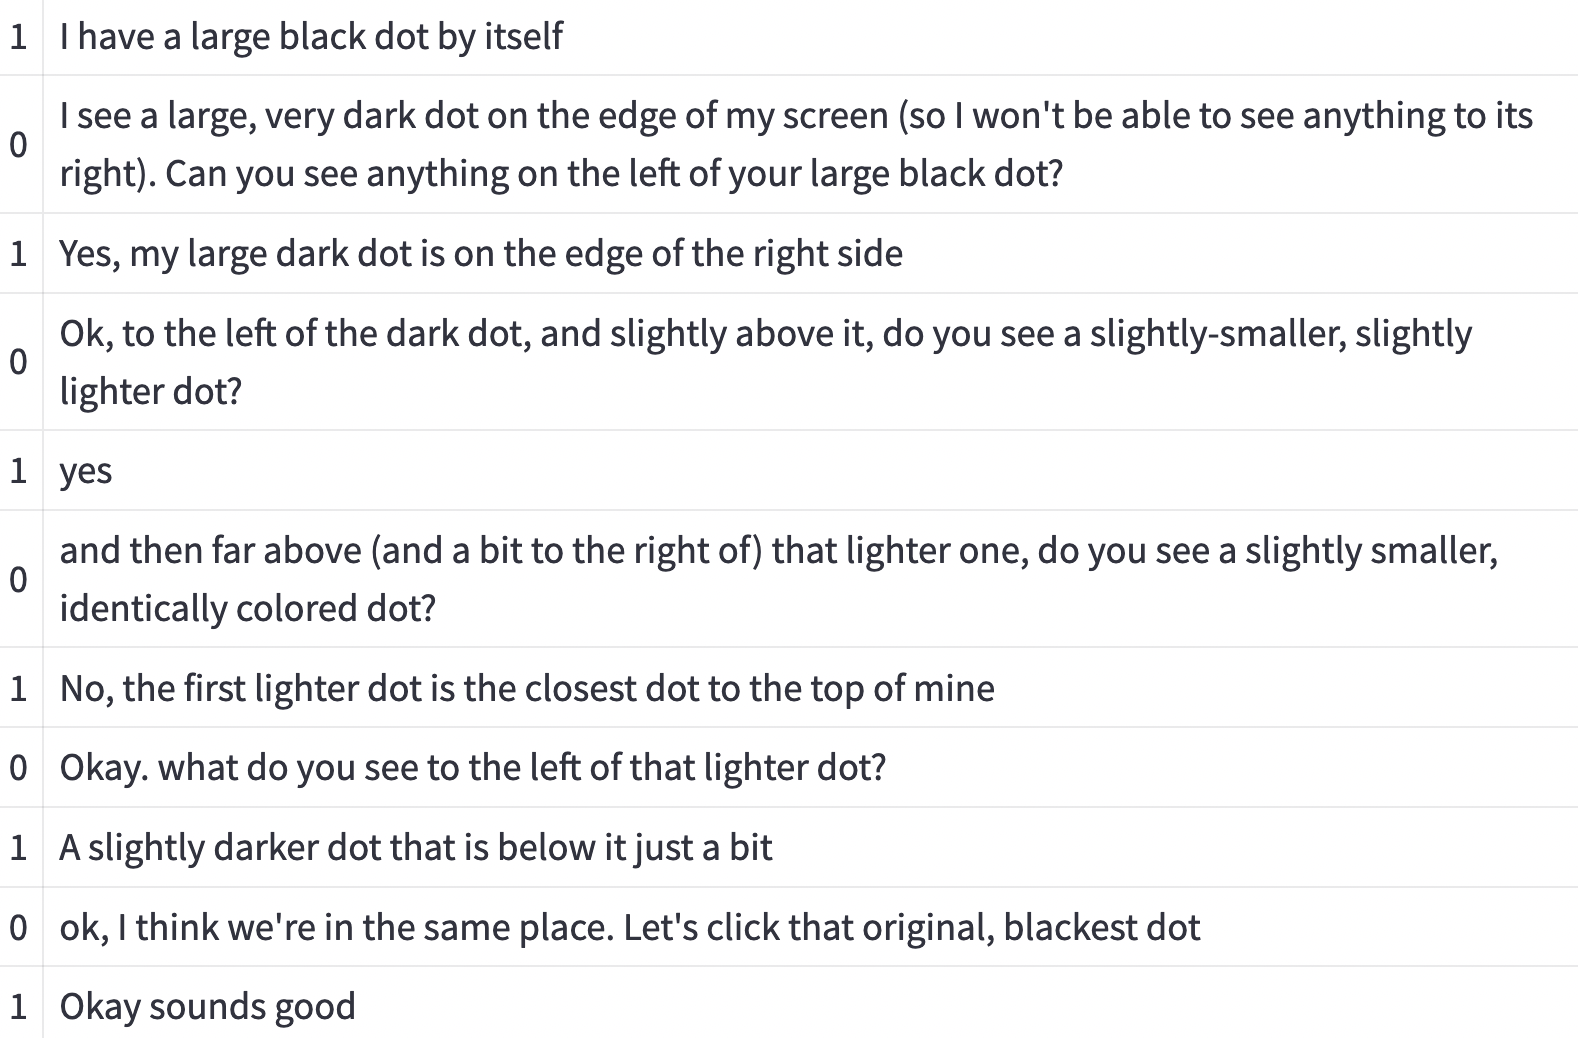
\includegraphics[width=\textwidth,clip,trim={0 9cm 0 0}]{img/words3.png}
\end{frame}

\begin{frame}
\frametitle{Example dialogue 3: Good humans}
\centering
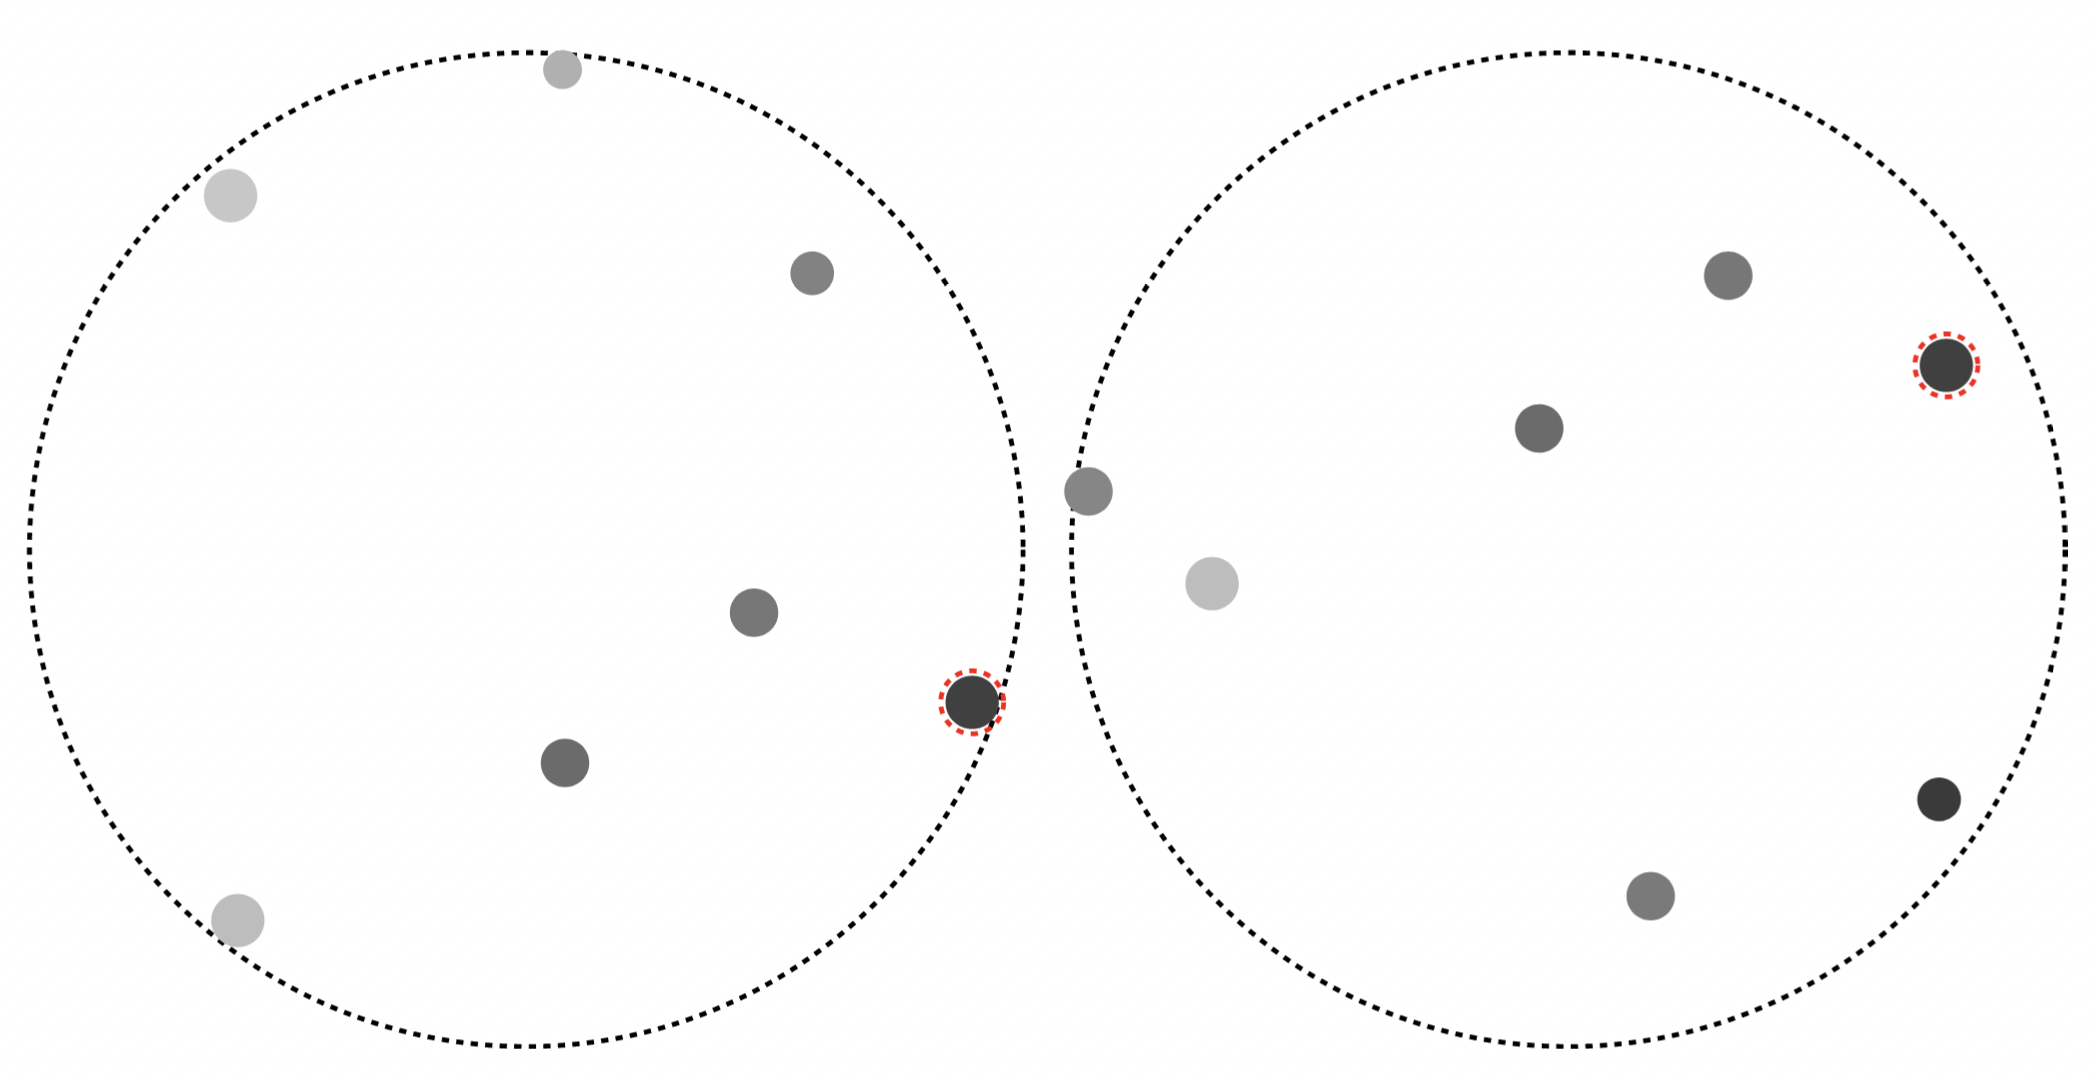
\includegraphics[width=0.75\textwidth]{img/dots3.png}
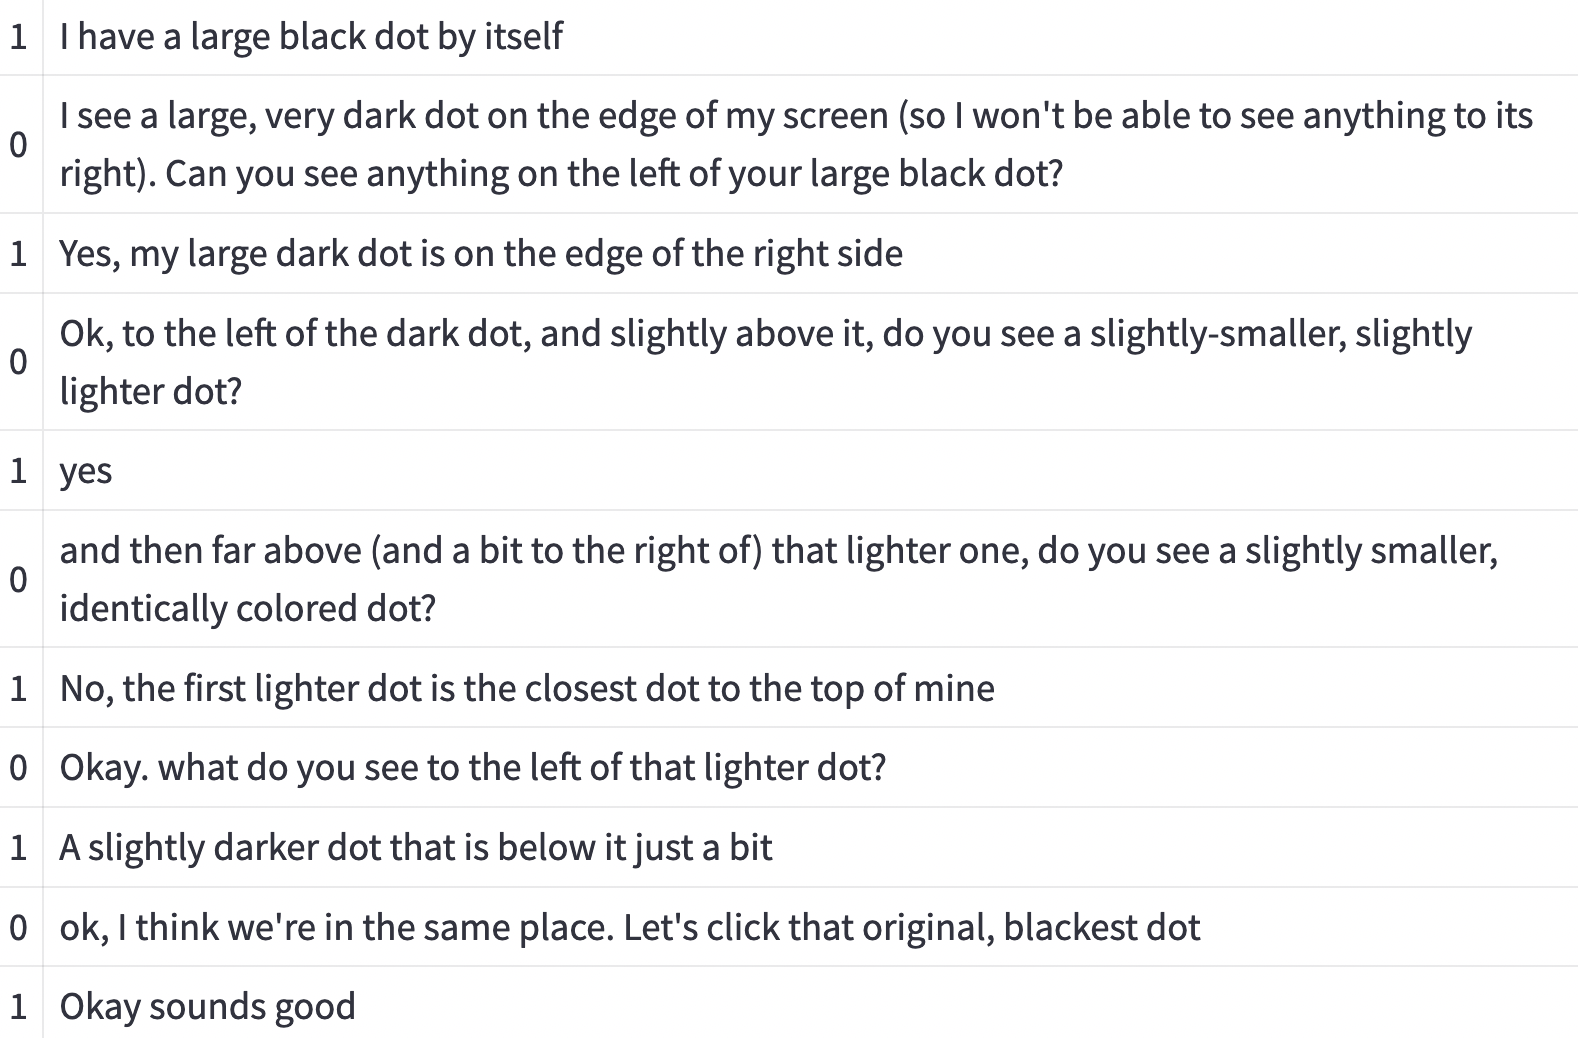
\includegraphics[width=\textwidth,clip,trim={0 0 0 9cm}]{img/words3.png}
\end{frame}



\end{document}
